\documentclass[fleqn]{jbook}
\usepackage{physpub}

\begin{document}

\begin{question}{教育 英語}{}

\begin{subquestions}
\SubQuestion
%次の2問について、別々の解答用紙に解答しなさい
%第1問
次の英文を読み、以下の設問に答えなさい
\baselineskip=12pt

 In 1961, during the very month that President John F. Kennedy launched the race to the moon, K. Watson, B. C. Murray and H. Brown of the California Institute of Technology noted the importance of the fact that some craters in the moon's polar regions are permanently in shadow. Rather then being subjected to two weeks of blistering rays from the sun each lunar month, these sites remain eternally dark and frigid. Such ``cold traps'', they argued, might snare water dumped on the lunar surface by crashing comets or spewed forth by lunar volcanoes. And over the aeons, inky crater floors near the poles might accumulate substantial amounts of ice. Those deposits would be immensely valuable to people on future lunar bases, who could distill water from them or separate out the oxygen and hydrogen to use as rocket propellant. It took nearly three decades, but the latest robot probe, Lunar Prospector, has seemingly confirmed that frozen caches of water can indeed be found on the moon.

 Because none of the Apollo missions visited the moon's poles, the \underline{(ア)proposal} of Watson, Murray and Brown had remained untested for 30 years. The first experimental indication came when the Department of Defense and National Aeronautics and Space Administration sent a probe called \underline{(a)Clementine} into a polar orbit around the moon in 1994.

 Clementine found evidence for ice by bouncing radar signals off the lunar surface and back to antennas on the earth. Some of the signals that were returned suggested that ice might be present near the moon's south pole. Yet Clementine uncovered no indications of ice at the north pole, even though the prove flew much lower there, and the radar experiment should have been more sensitive to ice on the surface.

 A 1994 report by the late \underline{(b)E. M. Shoemaker and two
 colleagues} at the U.S. Geological Survey noted that the south
 pole of the moon contains ``much larger'' areas of permanent shadow
 than the north does, although just how much was hard to say. So
 Clementine's finding evidence for ice only in the south seemed to
 make some sense. But in 1997 \underline{(c)three radio
 astronomers} reported that radar reflections of the type seen by
 Clementine could also be found for sunlit parts of the moon,
 casting doubt on this earlier indication of an icy southern
 pole. \underlineeng{(イ)And the latest results from Lunar Prospector
 have completely reversed the bias that had, up to this point, placed the moon's south pole in the spotlight.}

 According to \underline{(d)A. B. Binder} of the Lunar Research Institute, the leader of the Lunar Prospector science team, measurements from the spacecraft show ``about twice as much water ice in the north polar regions as in the south polar regions.'' Actually, the relevant instrument on Lunar Prospector can only sense the presence of hydrogen. The conclusion that the hydrogen detected is from water, Binder admits, is \underline{(ウ)``a leap of faith''} but a logical one. The ice is apparently mixed with a great deal of rock, so that it makes a tiny fraction of the lunar soil. However, the ice-tinged soil may extend a couple of meters deep.

 Binder does not yet know why the new results from Lunar Prospector show more ice in the north than in the south. He suggests that the shadow maps previously obtained from Clementine may have been misleading. Unfortunately the mystery remains unsolved for the moment: Lunar Prospector carries no camera, so the scientists cannot just take a quick look.\\
\\
snare:  捕らえる\\
spewed:  はき出される\\
aeons:  永遠\\
propellant:  (ロケット等の)推進剤\\
caches:  隠し場\\
leap:  跳躍\\

\baselineskip=15pt

\begin{subsubquestions}
\SubSubQuestion
下線部(ア)のproposalとは何か説明せよ
\SubSubQuestion
下線部(イ)を和訳せよ
\SubSubQuestion
下線部(ウ)にはどういう意味が込められているか。
\SubSubQuestion
下線部(a),(b),(c),(d)による主張点ないし観測結果を、その相互関係がわかるように要約せよ。
\end{subsubquestions}

\SubQuestion
つるまきバネ(coil spring)に重りをぶら下げると、その自然長から$x(m)$だけ伸びる。重りがバネに及ぼす力$F(N)$は、フックの法則(Hooke's law)より、$F=kx$と書ける。この時の比例定数$k(N/m)$をそのバネのバネ定数(spring constant)という。このフックの法則を確かめ、バネ定数kを測定する実験を行った。その測定結果は下図のグラフに$x$と$F$の関係として与えられている。\\
この実験を報告するレポートを英文で書け。ただし、 1.実験の目的、2.実験方法、3.結果、4.考察、5.結論 のセクションは、数行程度の記述で良い。必要ならば、解答用紙に適当な図を書き、それを参照しながら説明してもよい。\\
\begin{center}
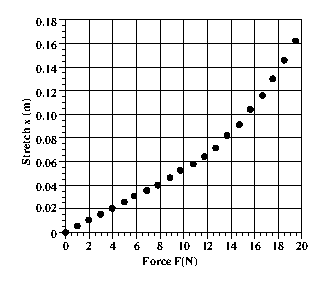
\includegraphics[clip,width=100mm]{1998eng2.eps}\\
{\Large Fig.~1}
\end{center}

\end{subquestions}
\end{question}
\begin{answer}{教育 英語}{}
\begin{subanswers}
\SubAnswer
  {\bf 全訳}

 1961年J.F.ケネディー大統領が月へのレースを始めました。その月にカルフォルニア工科大学のK.ワトソンとB.C.Murray、H.ブラウンの三人はいくつかの月の極地域のクレーターは永久に影になっているという事実の重要性に言及した。月の時間で毎月二週間、焼けつくような太陽光線にさらされないでこれらの地域は永久に暗く極寒のままである。彼らが議論するところによると、そのような「コールドトラップ」は彗星の衝突によって月の表面に投げ出された水や、月の火山の噴き出された水を捕らえ、長い間のち、極地方の真っ暗なクレーターの底に、大量の氷をため込んでいる可能性がある。その氷は未来の月面基地の人にとって非常に価値があり、蒸留して水を得たり、酸素と水素に分解してロケットの燃料に使ったりできる。30年近く経ったが、最新のロボット探査機「ルナ・プロスペクター」は、凍った水の場所を本当に月の上で見つけることができると、うわべでは確かめた。

 アポロ計画で月の極地方に訪れなかったので、3人の案は30年間手つかずに残った。最初の実験的兆候は国防総省とNASAが1994年に月の極軌道に送った探査機、クレメンタインを打ち上げたときに来た。

 クレメンタインは月の表面にレーダーを反射させて氷の証拠を得て、地球に送ってきた。帰ってきた信号のいくつかは氷が南極の近くにあるかも知れないということを示唆していた。しかし、クレメンタインは北極では南極より、より低く飛んでいるのにも関わらず、何の証拠も得られなかった。そして、レーダー実験は表面上の氷にもっと高感度にする方がよかった。

 アメリカ地質調査部の故シューメーカーと二人の同僚の1994年の報告は
どれくらいかは言い難いが、月の南極の方が、北極よりもより広い永久
の影を含むことを指摘した。そうすると、クレメンタインが南極でしか
氷の証拠を得られなかったのも理にかなうように思われた。しかし、
1997年、三人の電波天文学者は南極の氷のこの初期の証拠に疑いを投げ
かけ、クレメンタインに見られたレーダー反射のタイプは月の日が射す
部分によっても見られることを報告した。\underlinejpn{(イ)そして、月の探査機の最新の結果は、この時点まででは南極には日が射すという傾向に完全に戻ってしまった。}

 「月探査チーム」の指導者で、ルナリサーチ学会のA.B.Binderによると、宇宙船での測定は南極よりも北極の方が二倍の氷や水を示している。実際はルナ・プロスペクターの関連のある計器は水素の存在を感知するだけである。観測された水素が水からという結論はBinderも認めているが、論理的な結論でなく、飛躍がある。氷は大量の岩石と混ざっているらしく、月の土の小さなかけらになっている。しかし、氷を含んだ土は2〜3メートルの深さまで広がっているだろう。

 Binderは未だ「ルナ・プロスペクター」からの新しい証拠が南極より北極により多くの氷がある理由がわかっていない。Binderはクレメンタインから得られた過去の影の地図が間違っているのではないかと言うことを提案している。不幸なことに、今はその謎を解かずに残っている。ルナ・プロスペクターはカメラを持っていかなかったので、科学者は素早く見ることはできない。
\begin{subsubanswers}
\SubSubAnswer

月の極付近のクレーターは太陽の光が常に当たらないので、彗星の衝突や火山の噴火によって、月の表面に出た水を、氷としてため込んでいる可能性があり、その氷を未来の月面基地で利用するという案。

\SubSubAnswer
全訳を参照

\SubSubAnswer
水素の存在を感知しただけで、それが水からのものだと判断してしまう飛躍。

\SubSubAnswer
クレメンタインは月の表面から氷の存在を確認した。南極付近から氷の反応があり、北極付近からは何も反応がなかった。シューメーカー達の報告によれば、月の南極の方が北極よりも、より広い影がある。そうするとクレメンタインの結果が正しいように思える。しかし、三人の電波天文学者はクレメンタインの得た氷の反応は月の日が射す部分からも見られることを報告した。また、A.B.Binderによれば、ルナ・プロスペクターによる測定は、南極よりも北極の方が二倍の氷があり、クレメンタインによる観測とは全く逆になっている。
\end{subsubanswers}
\SubAnswer
ここにあげるのは一例。

\begin{subsubanswers}
\SubSubAnswer
\baselineskip=12pt

\begin{itemize}
\item Purpose

I  did  an experiment with a spring in order to make sure of Hooke's law
and obtain the spring constant of it.



\parbox[t]{110mm}{
\item Procedure

Fig.~2 shows the equipment of this experiment.


I hung a \( M\)[kg] weight from the lower end of the spring and measured 
the stretch \( x\)[m] of it.



\item Results

Fig.~1(the graph in the problem paper) shows the results.


Here \( F = Mg\)[N] is the value of the force pulling the spring and
\( g\)[m/\( s^{2}\)] is the gravitational acceleration.


And the self--weight of the spring is small enough by compared with \( M\).
So it was ignored.
}
\parbox[t]{60mm}{\vspace*{3mm}
\begin{center}
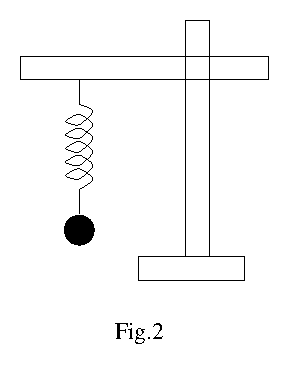
\includegraphics[clip,height=55mm,width=50mm]{1998engl.eps}
\end{center}
}

\item Consideration

From Fig.~1 when \( F\) is less than 10[N], Hooke's law is obviously valid.


But, otherwise \( F\) is not in proportion to \( x\).



\item Conclusion

A certain length \( x_{max}\) exists and \( F = kx\) (Hooke's law) is valid
for 


\( x < x_{max}\). And from Fig.~2, the spring constant \( k\)[N/m] is about 
194(for \( x \leq\) 0.06).

\end{itemize}


\SubSubAnswer

\begin{itemize}
\item The purpose of this experiment

I made sure of Hooke's law. I measured a spring constant \( k\).



\item The way of the experiment  Procedure

I hanged weight on a coil spring. I examined a relation between the
stretch \( x\) of the coilspring and the force \( F\) to pull the
coilspring.



\item The result

Fig.1 shows the relation between \( x\) and \( F\).



\item Consideration

If \( F\) is less than 12N, we find \( x\) and \( F\) follow Hooke's law.
The spring constant \( k\) is 1.8\( \times 10^{2}\)[N/m]. If \( F\) is 
stronger than 12N, \( x\) and \( F\) don't follow the law and \( F\) is
less than \( kx\).



\item Conclusion

We can conclude that if \( F\) is weak sufficiently, the coilspring follows
Hooke's law.

\end{itemize}
\SubSubAnswer

\begin{itemize}
\item Purpose

We make sure a coil spring follows Hooke's law and measure a spring constant
\( k\)[N/m].



\item Method

We hanged a weight from the coil spring and measure its stretch.



\item Result

Fig.1 shows the relationship between \( F\), which is the force given to the
coil spring and \( x\), which is the stretch of the coil spring.



\item Consideration

If \( F\) is smaller than about 12[N], the coil spring follows Hooke's law 
and the spring constant \( k\) is about 200[N/m].


If \( F\) is larger than about 12[N], \( x\) increases accelatirely and the
coil spring does not follow the hooke's law.



\item Conclusion

A coil spring follows Hooke's law when the force givn to it is small. But
if the force is large, it doesn't follow Hooke's law.

\end{itemize}

\SubSubAnswer
\begin{itemize}
\item Objective

The objective of this experiment is to confirm Hooke's law for a coil 
spring and measure the spring constant \( k\) of it.



\item Experimental Method

The stretch \( x\) of the coil spring was measured for various weights
having the different weight.



\item Result

Fig.1 provides a plot of \( x\) against the 
force \( F\) acting on the copil spring. From 
Fig.1 it can be stated that \( x\) increases 
almost linearly up to 10[N], above which it 
increases superlinearly.



\item Discussion

The result is consistent with Hooke's law up to 10[N]. Since 1/\( k\) is
equal to the slope of the fitted straight line Figure.~1, the spring constant
is 190[N/m].



\item Conclusion

\begin{itemize}
\item It is confirmed that Hooke's law is valid up to 10[N] for this coil
spring.
\item The spring constant of this spring is 190[N/m].
\end{itemize}
\end{itemize}

\baselineskip=15pt
\end{subsubanswers}

\end{subanswers}
\end{answer}


\end{document}